% Author Name: José Areia 
% Author Contact: jose.apareia@gmail.com
% Version: 1.0.3 - 18/04/2025
% Public Repository: https://github.com/joseareia/nob-article

% Packages & Document Configurations
\documentclass[twocolumn]{NobArticle}
\runninghead{Shortened Running Article Title}
\footertext{\textit{Journal X} (2023) 12:684}

% Title
\title{An Article Title That Spans Multiple Lines to Show Line Wrapping}

% Authors
\author{
    Author One\textsuperscript{1,2}, 
    Author Two\textsuperscript{3} 
    and Author Three\textsuperscript{1}
}

% Affiliations
\date{
    \textsuperscript{\textbf{1}}
    School of Computer Science, The University of City \\ \textsuperscript{\textbf{2}}
    Computer Science Department, The University of City \\ \textsuperscript{\textbf{3}}
    Computer Science Department, The University of Village
}

% Abstract
\renewcommand{\maketitlehookd}{%
\begin{abstract}
    \noindent Lorem ipsum dolor sit amet, consectetur adipiscing elit. Praesent porttitor arcu luctus, imperdiet urna iaculis, mattis eros. Pellentesque iaculis odio vel nisl ullamcorper, nec faucibus ipsum molestie. Sed dictum nisl non aliquet porttitor. Etiam vulputate arcu dignissim, finibus sem et, viverra nisl. Aenean luctus congue massa, ut laoreet metus ornare in. Nunc fermentum nisi imperdiet lectus tincidunt vestibulum at ac elit. Nulla mattis nisl eu malesuada suscipit. Aliquam arcu turpis, ultrices sed luctus ac, vehicula id metus. Morbi eu feugiat velit, et tempus augue. Proin ac mattis tortor. Donec tincidunt, ante rhoncus luctus semper, arcu lorem lobortis justo, nec convallis ante quam quis lectus. Aenean tincidunt sodales massa, et hendrerit tellus mattis ac. Sed non pretium nibh. Donec cursus maximus luctus. Vivamus lobortis eros et massa porta porttitor.
    
    \medskip

    \small{\textbf{Index Terms:} Keyword A, Keyword B, Keyword C.}
\end{abstract}
}

\begin{document}

\small
\maketitle

% Introduction
\section{Introduction}
\blindtext

% Contribution
\subsection{Contribution}
This paper as the follow contributions.

\begin{itemize}
	\item Arcu eros accumsan lorem, at posuere mi diam sit .
	\item Fusce fermentum, mi sit amet euismod rutrum.
	\item Sem lorem molestie diam, iaculis aliquet sapien tortor.
	\item Pellentesque bibendum pretium aliquet.
\end{itemize}

% Paper Organisation
\subsection{Paper Organisation}
\blindtext
\section{Background}
\blindtext

\subsection{Literature Review}
\blindtext This is a reference \citet{Elgamal1985} and this is another \citep{Elgamal1985}.
\section{Methods}
\blindtext

\begin{figure}[!htpb]
    \centering
    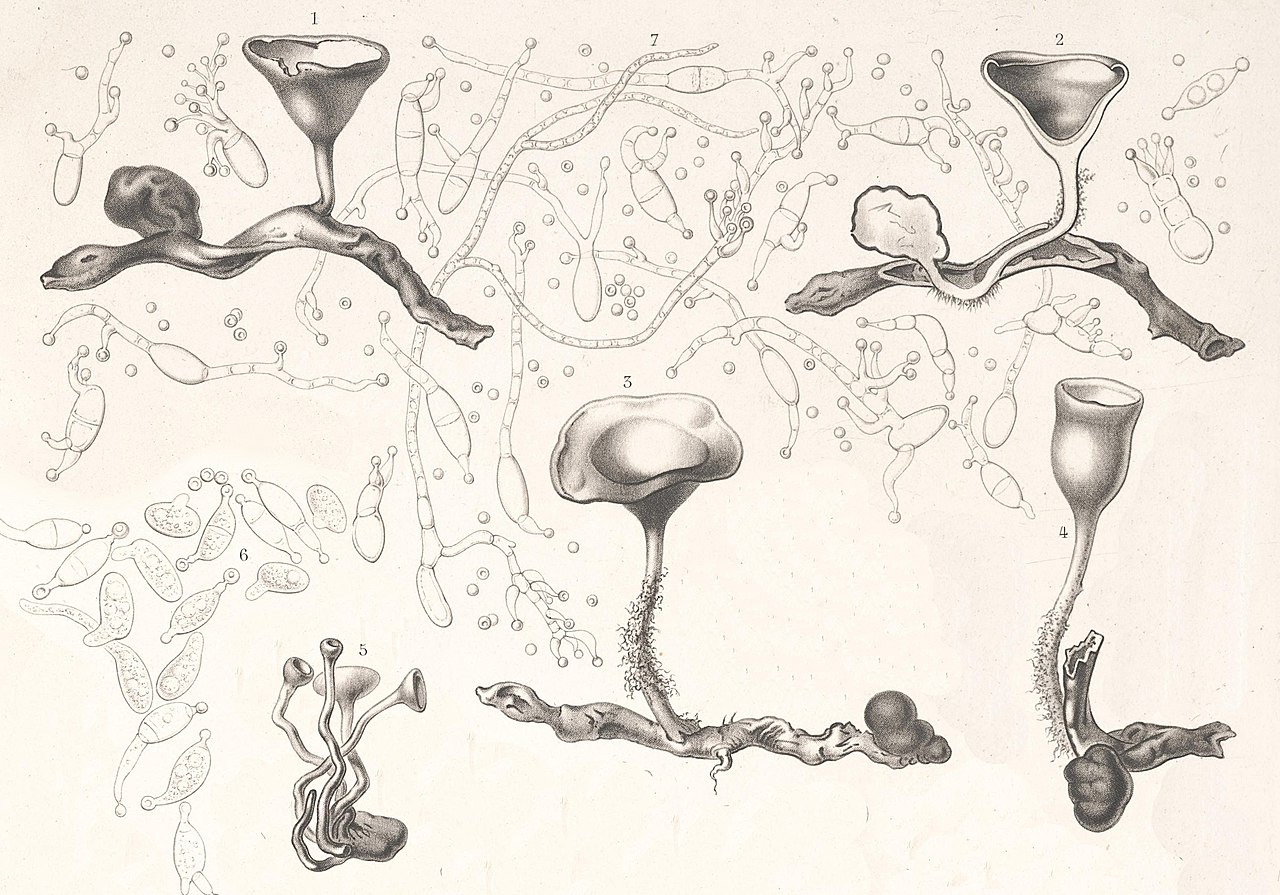
\includegraphics[width=\linewidth]{Figures/PezizaTuberosa.jpg}
    \caption{Illustration of the fungus Dumontinia tuberosa by physician, mycologist, and illustrator Charles Tulasne (1816–1884) in the book Selecta Fungorum Carpologia (1861–65). (Name of the original work: Peziza tuberosa parasite on Anemone nemorosa).}
    \label{fig:tcanther}
\end{figure}

\subsection{Method 01}
\blindtext

\subsubsection{Method 01.A}
\blindtext
% Results
\section{Results}
\blindtext

\begin{table}[!htpb]
    \caption{Floating point benchmark.
	\textbf{R$_{max}$}: the performance in GFlops for the largest problem run on a machine; \textbf{N$_{max}$}: the size of the largest problem run on a machine; \textbf{N$_{1/2}$}: the size where half the \textbf{R$_{max}$} execution rate is achieved; \textbf{R$_{peak}$}: the theoretical peak performance in GFlops.}
    \label{tab:table-01}
    \centering
    \begin{tabularx}{\linewidth}{rcccc}
        \toprule
        \textbf{Linpack	Benchmark}& Proc. & \textbf{R$_{max}$} & \textbf{N$_{max}$} & \textbf{R$_{peak}$} \\ 
        (Full precision) & or Cores	& GFlops & Order & GFlops \\ [0.25ex] 
        \midrule
        Thinking Machine CM-5 & 32 & 1,900 & 9216 & 4 \\
        Pentium 4 3.0 GHz & 1 & 4,730 & 7600 & 6 \\
        \multirow{2}{*}{IBM Cell BE 3.2 GHz} & \multirow{2}{*}{9} & \multirow{2}{*}{98,05} & \multirow{2}{*}{4096} & 204,8 \scriptsize{(32b)} \\
        & & & & 14,6 \scriptsize{(64b)} \\
        Thinking Machine SD-3 & 36 & 1,120 & 6728 & 3 \\
        \bottomrule
    \end{tabularx}
\end{table}
% Discussion
\section{Discussion}
\blindtext
% Conclusion
\section{Conclusion}
\blindtext

\section*{Acknowledgements}
This research received support during the XXX course, instructed by Professor XXX, PhD at the School of XXX, XXX.

\printbibliography

\end{document}